\documentclass{article}
\usepackage[utf8]{inputenc}
\usepackage{amsmath,amssymb,mathtools}
\usepackage{amsthm}
\usepackage{thmtools}
\usepackage{hyperref}
% `cleveref` has to be loaded after `hyperref`
\usepackage{cleveref}
\usepackage{stackengine}
\usepackage{minted}
\usepackage{tcolorbox}
\usepackage{multicol}
\usepackage{prftree}
\usepackage{fancyvrb}
\usepackage{csquotes}
\usepackage{appendix}

\title{Cartesian Reachability Logic}
\author{Jan Tušil }
\date{February 2022}

\declaretheorem[]{example}
\declaretheorem[]{definition}
\declaretheorem[]{lemma}
\declaretheorem[]{theorem}
\declaretheorem[]{remark}

\newcommand{\RL}{\mathsf{RL}}
\newcommand{\ML}{\mathsf{ML}}
\newcommand{\CRL}{\mathsf{CRL}}
\newcommand{\Var}{\mathit{Var}}
\newcommand{\Tcfg}{\mathcal{T}_{\mathit{Cfg}}}

\newcommand\oast{\stackMath\mathbin{\stackinset{c}{0ex}{c}{0ex}{\ast}{\bigcirc}}}

\begin{document}

\maketitle

\section{Introduction}

\section{Preliminaries}

\subsection{($\mu$-free) Matching Logic}

\subsection{One-path Reachability Logic}



\begin{definition}[\cite{StefanescuCMMSR19}]
We define reachability-logic signatures, rules, and systems as follows.
\begin{enumerate}
    \item A reachability-logic \emph{signature} is a pair $(\Sigma, \mathit{Cfg})$,
          where $\Sigma$ is a matching logic signature and $\mathit{Cfg}$ is a sort.
          
    \item A \emph{one-path reachability rule} over reachability logic signature $(\Sigma, \mathit{Cfg})$        is a pair $\varphi \Rightarrow^\exists \varphi^\prime$,
          where $\varphi$ and $\varphi^\prime$
          are patterns (which can have free variables) of sort $\mathit{Cfg}$.
          
    \item A \emph{reachability system} over a reachability-logic signature $(\Sigma, \mathit{Cfg})$
          is a pair $\mathcal{S} = (\mathcal{T}, S)$, where $\mathcal{T}$ is a $\Sigma$-algebra
          and $S$ is a set of reachability rules over $(\Sigma, \mathit{Cfg})$.
          
    \item A rule $\varphi \Rightarrow^\exists \varphi^\prime$ over $(\Sigma, \mathit{Cfg})$
          is \emph{weakly well-defined}
          with respect to $\Sigma$-algebra $\mathcal{T}$
          iff
          for any $\gamma \in \Tcfg$ and $\rho : \Var \to \mathcal{T}$
          with $(\gamma, \rho) \vDash \varphi$,
          there exists $\gamma^\prime \in \Tcfg$ with $(\gamma^\prime , \rho) \vDash \varphi^\prime$.
          
    \item A reachability system $\mathcal{S}$ is \emph{weakly well-defined} iff each its rule is weakly     
          well-defined.
          
    \item A reachability system $\mathcal{S} = (\mathcal{T}, S)$ over $(\Sigma, \mathit{Cfg})$ induces
          a \emph{transition system} \\
          $(\Tcfg , \Rightarrow_{\mathcal{S}})$,
          where $\gamma \Rightarrow_{\mathcal{S}} \gamma^\prime$
          for $\gamma, \gamma^\prime \in \Tcfg$
          iff there is some rule \\ $\varphi \Rightarrow^\exists \varphi^\prime \in S$
          and some valuation $\rho : \Var \to \mathcal{T}$ with $(\gamma, \rho) \vDash \varphi$
          and $(\gamma^\prime , \rho) \vDash \varphi^\prime$.

    \item A reachability system $(\mathcal{T}, S)$ is \emph{deterministic} iff the induced transition system
          is deterministic.

    \item A configuration $\gamma \in \Tcfg$ \emph{terminates} in $(\Tcfg , \Rightarrow_{\mathcal{S}})$
          iff there is no infinite $\Rightarrow_{\mathcal{S}})$-sequence starting with $\gamma$.
          
    \item A \emph{$\Rightarrow_{\mathcal{S}}$-path} is a finite
          sequence $\gamma_0 \Rightarrow_{\mathcal{S}} \gamma_1 \Rightarrow_{\mathcal{S}} \ldots
          \Rightarrow_{\mathcal{S}} \gamma_n$
          with $\gamma_0,\ldots,\gamma_n \in \Tcfg$.
          
    \item A $\Rightarrow_{\mathcal{S}}$-path is \emph{complete}
          iff it is not a strict prefix of any
          other $\Rightarrow_{\mathcal{S}}$-path.

    \item A \emph{one-path reachability rule}
          is a pair $\varphi \Rightarrow^\exists \varphi^\prime$ of patterns $\varphi$ and $\varphi^\prime$.

    \item A one-path reachability rule $\varphi \Rightarrow^\exists$ is \emph{satisfied}
          in a reachability system $\mathcal{S}$,
          written $\mathcal{S} \vDash_\RL \varphi \Rightarrow^\exists \varphi^\prime$,
          iff for every $\gamma \in \Tcfg$
          such that $\gamma$ terminates in $(\Tcfg, \Rightarrow_{\mathcal{S}})$
          and for any valuation $\rho : \Var \to \mathcal{T}$
          such that $(\gamma, \rho) \vDash \varphi$,
          there exists some $\gamma^\prime \in \Tcfg$
          such that
          and $(\gamma^\prime, \rho) \vDash \varphi^\prime$

%    \item An all-path reachability rule $\varphi \Rightarrow^\forall$ is \emph{satisfied},
%          written $\mathcal{S} \vDash_\RL \varphi \Rightarrow^\forall \varphi^\prime$,
%          iff for all complete $\Rightarrow_{\mathcal{S}}$-paths $\tau$
%          starting with $\gamma \in \Tcfg$ and for all $\rho : \Var \to \mathcal{T}$
%          such that $(\gamma, \rho) \vDash \varphi$,
%          there exists some $\gamma^\prime \in \tau$
%          such that $(\gamma^\prime, \rho) \vDash \varphi^\prime$.
\end{enumerate}

\begin{figure}
    \centering
    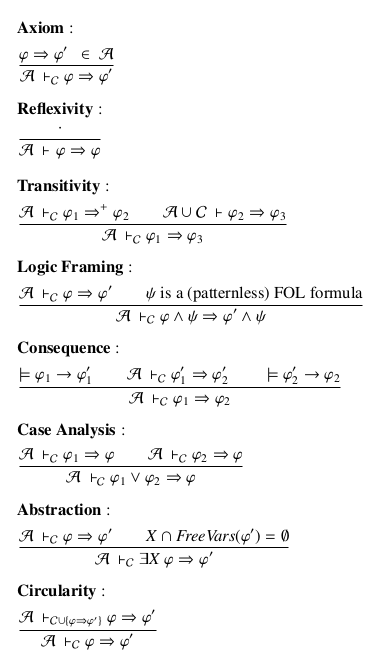
\includegraphics[width=0.5\textwidth]{img/onepath-rl.png}
    \caption{One-path reachability-logic proof system.
    The use of $\Rightarrow^+$ in sequent means that it was derived without Reflexivity.
    TODO retypeset}
    \label{fig:RLproofsystem}
\end{figure}

We have RL sequents of the shape $\mathcal{T}, A, C \vdash_\RL \varphi \Rightarrow^\exists \varphi^\prime$.

\end{definition}

\section{Cartesian Reachability Logic}

We need to make the definition such that it works with reachability logic for the composite semantics.
Here is one attempt:
\begin{definition}\label{def:CRLsemantics}
A Cartesian reachability rule
$(\varphi_1,\ldots,\varphi_k) \land \varphi \Rightarrow^{c\exists} (\psi_1,\ldots,\psi_k) \land \psi$
of arity $k$
is \emph{valid} in a reachability system $(\mathcal{T}, S)$,
written
$(\mathcal{T}, S) \vDash_\CRL (\varphi_1,\ldots,\varphi_k) \land \varphi \Rightarrow^{c\exists}
(\psi_1,\ldots,\psi_k) \land \psi$,
iff for all configurations $\sigma_1,\ldots,\sigma_k \in \Tcfg$ and any $\mathcal{T}$-valuation $\rho$,
whenever $\sigma_1 \in |\varphi_1 \land \varphi|_\rho \land \ldots \land \sigma_k \in |\varphi_l \land \varphi|_\rho$,
then for every $k$-tuple complete paths $(\pi_1, \ldots, \pi_k)$
of respective lengths $l_1, \ldots, l_k$
such that
$\sigma_1 = \pi_1(0) \land \ldots \land \sigma_k = \pi_k(0)$,
it holds that 
$\pi_1(l_1-1) \in |\varphi_1 \land \psi|_\rho \land \ldots \land \pi_k(l_k-1) \in |\varphi_k \land \psi|_\rho$.
\end{definition}

TODOs:
\begin{itemize}
    \item Validate this definition against examples from the CHL paper.
    \item Have a "running example" - some programming language, like IMP?
    \item Have an example how do we perform lockstep execution on ifs.
    \item Conservativeness argument for the additional rules?
\end{itemize}

\begin{definition}
We translate a language semantics into a semantics for lists of configurations as follows.
\begin{enumerate}
    \item Let $(\Sigma, \mathit{Cfg})$ be a reachability-logic signature.
          Then $(\Sigma, \mathit{Cfg})^*$ = $(\Sigma^*, \mathit{Cfg}^*)$,
          where
          \begin{enumerate}
              \item $\Sigma^* = \Sigma \cup \{ \mathit{cfgitem}, \mathit{cfgconcat},
          %\mathit{cfgdummy},
          \mathit{cfgheat} \}$
              \item $\mathit{Cfg}^*$ is a fresh sort (representing the sort of lists of configurations);
              %\item $\mathit{cfgdummy}$ is a fresh symbol of sort $\mathit{Cfg}$;
              \item $\mathit{cfgitem}$ a fresh symbol of sort $\mathit{Cfg} \to \mathit{Cfg}^*$;
              \item $\mathit{cfgconcat}$ a fresh symbol of sort $\mathit{Cfg}^* \times \mathit{Cfg}^* \to \mathit{Cfg}^*$; and
              \item $\mathit{cfgheat}$ is a fresh symbol of sort $\mathit{Cfg}^* \times \mathit{Cfg} \times \mathit{Cfg}^* \to \mathit{Cfg}^*$.
          \end{enumerate}
    \item Let $S$ be a set of reachability rules over $(\Sigma, \mathit{Cfg})$.
          We generate a set of reachability rules $S^*$ over $(\Sigma, \mathit{Cfg})^*$
          by setting
          \begin{equation*}
              S^* = \{ \mathit{cfgheat}(L, \varphi_1, R) \Rightarrow^\exists \mathit{cfgheat}(L, \varphi_2, R) \mid (\varphi_1 \Rightarrow^\exists \varphi_2) \in S \} \, ,
          \end{equation*}
          where $L,R$ are distinct fresh variables (not occurring in any rule in $S$).
    \item Let $\mathcal{T}$ be a configuration model; that is, a $\Sigma$-algebra.
          We generate a $\Sigma^*$-algebra $\mathcal{T}*$, which interprets all sorts and symbols from
          $\Sigma$ as in $\mathcal{T}$, and in addition interprets
          \begin{enumerate}
              \item the sort $\mathit{Cfg}*$ as the set of all finite lists
              $[c_1;\ldots;c_n]$ for $n \in \mathbb{N}$, where $c_i$ is an element of sort $\mathit{Cfg}$
              for any $0 \leq i \leq n$;
              \item the symbol $\mathit{cfgitem}$ as the function $\lambda c.\, [c]$;
              \item the symbol $\mathit{cfgconcat}$ as the function $\lambda l_1,l_2.\, l_1 \texttt{++} l_2$,
                where $\texttt{++}$ is list concatenation; and
              \item the symbol $\mathit{cfgheat}$ as the function
                $\lambda l_1, c, l_2.\, l_1 \texttt{++} [c] \texttt{++} l_2$.
          \end{enumerate}
          
    \item Let $\mathcal{S} = (\mathcal{T}, S)$ be a reachability system over $(\Sigma, \mathit{Cfg})$.
          We generate a reachability system $\mathcal{S}^*$ over $(\Sigma, \mathit{Cfg})^*$
          by setting $\mathcal{S}^* = (\mathcal{T}^*, S^*)$.
\end{enumerate}
\end{definition}

\begin{lemma}
    The star extension on matching logic models is conservative.
\end{lemma}
\begin{proof}
Admitted.
\end{proof}

\begin{lemma}
    Let $\mathcal{S} = (\mathcal{T}, S)$ be a reachability-logic system over $(\Sigma, \mathit{Cfg})$.
    For any $k \geq 1$, any configurations $c_1,\ldots,c_k, c^\prime \in \Tcfg$, and any $1 \leq i \leq k$,
    we have
    \begin{equation*}
        c_i \Rightarrow_{\mathcal{S}} c^\prime
                    \iff
        [c_1,\ldots,c_k] \Rightarrow_{\mathcal{S}^*} [c_1, \ldots, c_{i-1}, c^\prime, c_{i+1}, \ldots, c_k]
    \end{equation*}
\end{lemma}
\begin{proof}
Admitted.
\end{proof}


\section{Proof System}

The proof system derives claims of the shape
$\mathcal{S}, \vdash_\CRL (\varphi_1, \ldots, \varphi_k) \land P \Downarrow_{C,E} \Psi$,
where $P$ is a patternless FOL formula.
The idea is that $P$ is the part of the claim that relates variables from different components.
Initially, the proof starts with the claim
$\mathcal{S} \vdash_\CRL (\varphi_1, \ldots, \varphi_k) \land P \Downarrow_{\emptyset, \emptyset} \Psi$.

\begin{definition}
We define $\mathit{mergePatterns}$ and $\mathit{flatten}$ as follows:
\begin{enumerate}
    \item $\mathit{mergePatterns}(\varphi) = \mathit{cfgitem}(\varphi)$;
    \item $\mathit{mergePatterns}(\varphi_1, \varphi_2, \ldots, \varphi_n)
        = \mathit{cfgconcat}(\mathit{cfgitem}(\varphi_1), \mathit{mergePatterns}(\varphi_2, \ldots, \varphi_n))$ for $n \geq 2$; and
    \item $\mathit{flatten}((\varphi_1, \ldots, \varphi_k) \land P)
        = \mathit{mergePatterns}(\varphi_1, \ldots, \varphi_k) \land P$.
    \item $\mathit{flatten}^\exists(\Psi, \Psi^\prime) = \mathit{flatten}(\Psi) \Rightarrow^\exists \mathit{flatten}(\Psi^\prime)$
    \item $\mathit{flatten}^\exists(A, \Psi^\prime) = \{ \mathit{flatten}^\exists(\Psi, \Psi^\prime) \mid \Psi \in A \}$, where $A$ is a set.
\end{enumerate}
\end{definition}

\begin{figure}
    \centering
    \begin{align*}
    & \prftree[l]{Reflexivity}{\mathcal{S} \vdash_\CRL \Psi \Downarrow_{\emptyset,E} \Psi}
    \end{align*}
    \begin{align*}
    & \prftree[l]{Axiom}{\Psi \in E}{\mathcal{S} \vdash_\CRL \Psi \Downarrow_{C,E} \Psi^\prime}
    \end{align*}
    \begin{align*}
    & \prftree[l]{Reduce}
      {(\mathcal{T}^*, S^* \cup \mathit{flatten}^\exists(E, \Psi^\prime)), \emptyset \vdash_\RL
        \mathit{flatten}^\exists(\Psi, \Psi^\prime) }
      {(\mathcal{T}, S) \vdash_\CRL \Psi \Downarrow_{C,E} \Psi^\prime}
    \end{align*}
    \begin{align*}
    & \prftree[l]{Case}
    { \prfStackPremises
      {\mathcal{S} \vdash_\CRL (\varphi_1, \ldots, \varphi_{i-1}, \varphi_i, \varphi_{i+1}, \ldots, \varphi_k) \land P^\prime \Downarrow_{C, E} \Psi^\prime }
      {\mathcal{S} \vdash_\CRL (\varphi_1, \ldots, \varphi_{i-1}, \psi_i, \varphi_{i+1}, \ldots, \varphi_k) \land P^\prime \Downarrow_{C, E} \Psi^\prime }
    }
    {\mathcal{S} \vdash_\CRL (\varphi_1, \ldots, \varphi_{i-1}, (\varphi_i \lor \psi_i), \varphi_{i+1}, \ldots, \varphi_k) \land P^\prime \Downarrow_{C, E} \Psi^\prime}
    \end{align*}
    \begin{align*}
    & \prftree[l]{Step}
    { \prfStackPremises
       {\varphi \Rightarrow^\exists \varphi^\prime \in S}
       {\mathcal{T} \vDash_\ML \varphi_i \leftrightarrow (\varphi \land \psi)}
       {\psi \mbox{ is a patternless FOL formula}}
       %{ \mathcal{S}^* \vDash_\RL \varphi_i \Rightarrow^{\forall+} \varphi_i^\prime }
       {  (\mathcal{T}, S) \vdash_\CRL (\varphi_1, \ldots, \varphi_{i-1}, \varphi^\prime \land \psi, \varphi_{i+1}, \ldots, \varphi_k)
          \land P
          \Downarrow_{\emptyset, (C \cup E)} \Psi^\prime
      }
    }
    {(\mathcal{T}, S) \vdash_\CRL (\varphi_1, \ldots, \varphi_{i-1}, \varphi_i, \varphi_{i+1}, \ldots, \varphi_k) \land P \Downarrow_{C, E} \Psi^\prime}
    \end{align*}
    \begin{align*}
    & \prftree[l]{Circularity}
      { \mathcal{S} \vdash_\CRL \Psi \Downarrow_{C \cup \{ \Psi \} , E} \Psi^\prime}
      { \mathcal{S} \vdash_\CRL \Psi \Downarrow_{C, E} \Psi^\prime}
    \end{align*}
    \begin{align*}
    & \prftree[l]{Conseq}
      { \prfStackPremises
        { (\mathcal{T}, S) \vdash_\CRL \Phi^\prime \Downarrow_{C, E} \Psi^\prime}
        { \mathcal{T}^* \vDash_\ML \mathit{flatten}(\Phi) \leftrightarrow \mathit{flatten}(\Phi^\prime) }
      }
      { (\mathcal{T}, S) \vdash_\CRL \Phi \Downarrow_{C, E} \Psi^\prime}
    \end{align*}
%    \begin{align*}
%    & \prftree[l]{Conseq2}
%      { \prfStackPremises
%        { (\mathcal{T}, S) \vdash_\CRL (\varphi_1, \ldots, \varphi_k) \land P \Downarrow_{C, E} \Psi^\prime}
%        { \mathcal{T} \vDash_\ML \varphi_i \leftrightarrow \psi_i }
%      }
%      { (\mathcal{T}, S) \vdash_\CRL (\varphi_1^\prime, \ldots, \varphi_{i-1}, \varphi_{i}, \varphi_{i+1}, \ldots, \varphi_k^\prime) \land P^\prime \Downarrow_{C, E} \Psi^\prime}
%    \end{align*}
    \caption{Proof System}
    \label{fig:my_label}
\end{figure}



\begin{lemma}
    \begin{equation*}
        (\mathcal{T}, S) \vdash_\CRL \Psi \Downarrow_{C,E} \Psi^\prime
        \implies
        (\mathcal{T}^*, S^* \cup \mathit{flatten}^\exists(E, \Psi^\prime)), \mathit{flatten}^\exists(C, \Psi^\prime) \vdash_\RL
          \mathit{flatten}^\exists(\Psi, \Psi^\prime) 
    \end{equation*}
\end{lemma}
\begin{proof}
By induction on the structure of the CRL proof. TODO
\begin{enumerate}
    \item If the proof ends with \emph{Reduce}, then we are done, since $\mathit{flatten}^\exists(\emptyset, \psi^\prime) = \emptyset$.
    
    \item If the proof ends with \emph{Reflexivity}, then we need to prove
    \begin{equation*}
        \mathcal{S}^*, \mathit{flatten}^\exists(E, \psi), \emptyset \vdash_\RL
          \mathit{flatten}^\exists(\psi, \psi) 
    \end{equation*}
    which we do by applying the Reflexivity proof rule.
    
    \item If the proof ends with \emph{Axiom}, then $\psi \in E$,
          and we have to prove that
          \begin{equation*}
            \mathcal{S}^*, \mathit{flatten}^\prime(E, \psi^\prime), \mathit{flatten}^\prime(C, \psi^\prime) \vdash_\RL
            \mathit{flatten}^\prime(\psi, \psi^\prime)               \, .
          \end{equation*}
          By applying the Axiom proof rule of RL, it is enough to show that
          \begin{equation*}
              \mathit{flatten}^\prime(\psi, \psi^\prime) \in \mathit{flatten^\prime}(E, \psi^\prime) \, ,
          \end{equation*}
          which follows from $\psi \in E$.
          
    \item If the proof ends with \emph{Case}, then we have
        \begin{equation*}
            \mathcal{S}^*, \Bar{E}, \Bar{C} \vdash_\RL
            \mathit{flatten}^\exists((\varphi_1, \ldots, \varphi_{i-1}, \varphi_i, \varphi_{i+1}, \ldots, \varphi_k) \land P^\prime, \Psi^\prime)
        \end{equation*}
        and
        \begin{equation*}
            \mathcal{S}^*, \Bar{E}, \Bar{C} \vdash_\RL
            \mathit{flatten}^\exists((\varphi_1, \ldots, \varphi_{i-1}, \psi_i, \varphi_{i+1}, \ldots, \varphi_k) \land P^\prime, \Psi^\prime) 
        \end{equation*}
        as hypotheses, and we have to prove
        \begin{equation*}
            \mathcal{S}^*, \Bar{E}, \Bar{C} \vdash_\RL
            \mathit{flatten}^\exists((\varphi_1, \ldots, \varphi_{i-1}, (\varphi_i \lor \psi_i), \varphi_{i+1}, \ldots, \varphi_k) \land P^\prime, \Psi^\prime)               \, .
        \end{equation*}
        (where $\Bar{E} = \mathit{flatten}^\exists(E, \psi^\prime)$
         and $\Bar{C} = \mathit{flatten}^\exists(C, \psi^\prime)$
        ).
        After simplifications, we get
        \begin{align*}
            \mathcal{S}^*, \Bar{E}, \Bar{C} \vdash_\RL
            &
            \mathit{mergePatterns}((\varphi_1, \ldots, \varphi_{i-1}, \varphi_i, \varphi_{i+1}, \ldots, \varphi_k)) \land P^\prime
            \\ & \Rightarrow^\exists
            \mathit{flatten}(\Psi^\prime)
        \end{align*}
        and
        \begin{align*}
            \mathcal{S}^*, \Bar{E}, \Bar{C} \vdash_\RL
            &
            \mathit{mergePatterns}((\varphi_1, \ldots, \varphi_{i-1}, \psi_i, \varphi_{i+1}, \ldots, \varphi_k)) \land P^\prime
            \\ & \Rightarrow^\exists
            \mathit{flatten}(\Psi^\prime)
        \end{align*}
        as hypotheses,
        and have to prove
        \begin{align*}
            \mathcal{S}^*, \Bar{E}, \Bar{C} \vdash_\RL
            &
            \mathit{mergePatterns}((\varphi_1, \ldots, \varphi_{i-1}, (\varphi_i \lor \psi_i), \varphi_{i+1}, \ldots, \varphi_k)) \land P^\prime
            \\ & \Rightarrow^\exists
            \mathit{flatten}(\Psi^\prime)
        \end{align*}
        Since
        \begin{align*}
            \mathcal{T}^* \vDash_\ML & \mathit{mergePatterns}((\varphi_1, \ldots, \varphi_{i-1}, (\varphi_i \lor \psi_i), \varphi_{i+1}, \ldots, \varphi_k)) \land P^\prime \leftrightarrow \\
            & (\mathit{mergePatterns}((\varphi_1, \ldots, \varphi_{i-1}, \varphi_i, \varphi_{i+1}, \ldots, \varphi_k)) \land P^\prime \\
            & \lor \mathit{mergePatterns}((\varphi_1, \ldots, \varphi_{i-1}, \psi_i, \varphi_{i+1}, \ldots, \varphi_k)) \land P^\prime)
        \end{align*}
        (where $\mathcal{S}^* = (\mathcal{T}^*, S)$),
        we can apply the Consequence RL rule on the goal, followed by a Case Analysis rule applied to the two hypotheses, and we are done.
        
    \item If the proof ends with \emph{Step},
      we can assume a patternless FOL formula $\psi$, a rule $\varphi \Rightarrow^\exists \varphi^\prime \in S$ such that
      $\mathcal{T} \vDash_\ML \varphi_i \leftrightarrow (\varphi \land \psi)$,
      and an induction hypothesis
      \begin{align*}
        (&\mathcal{T}^*, S^* \cup \mathit{flatten}^\exists(C \cup E, \Psi^\prime)), \emptyset \vdash_\RL
          \\ &
          \mathit{flatten}((\varphi_1, \ldots, \varphi_{i-1}, \varphi^\prime \land \psi, \varphi_{i+1}, \ldots, \varphi_k) \land P) \Rightarrow^\exists \mathit{flatten}(\Psi^\prime)     
      \end{align*}
      and have to construct
      \begin{align*}
      & (\mathcal{T}^*, S^* \cup \mathit{flatten}^\exists(E, \Psi^\prime)), \mathit{flatten}^\exists(C, \Psi^\prime) \vdash_\RL \\
          & \mathit{flatten}((\varphi_1, \ldots, \varphi_{i-1}, \varphi_i, \varphi_{i+1}, \ldots, \varphi_k) \land P) \Rightarrow^\exists \mathit{flatten}(\Psi^\prime)    \, .
      \end{align*}
      
    We apply the Transitivity rule with the second premise being our first inductive hypothesis, and it remains to prove the second premise, which is (after simplification)
    \begin{align*}
        & (\mathcal{T}, S)^*, \mathit{flatten}^\prime(E, \psi^\prime), \mathit{flatten}^\prime(C, \psi^\prime)
        \\& \vdash_\RL
        (\mathit{mergePatterns}(\varphi_1, \ldots, \varphi_{i-1}, \varphi_i, \varphi_{i+1}, \ldots,                          \varphi_k) \land P)
        \\&\quad \Rightarrow^\exists
        (\mathit{mergePatterns}(\varphi_1, \ldots, \varphi_{i-1}, (\varphi^\prime \land \psi), \varphi_{i+1}, \ldots, \varphi_k) \land P) \, .
    \end{align*}
    By Congruence lemma and our assumption $\mathcal{T} \vDash_\ML \varphi_i \leftrightarrow (\varphi \land \psi)$ (adding the star does not break anything, by conservativeness), we have
    \begin{align*}
        \mathcal{T}^* \vDash_\ML &
        (\mathit{mergePatterns}(\varphi_1, \ldots, \varphi_{i-1}, \varphi_i, \varphi_{i+1}, \ldots,                          \varphi_k) \land P)
        \\ & \leftrightarrow
        (\mathit{mergePatterns}(\varphi_1, \ldots, \varphi_{i-1}, (\varphi \land \psi), \varphi_{i+1}, \ldots, \varphi_k) \land P) \, ,
    \end{align*}
    and therefore we can apply the Consequence rule on the goal, changing it into
    \begin{align*}
        & (\mathcal{T}, S)^*, \mathit{flatten}^\prime(E, \psi^\prime), \mathit{flatten}^\prime(C, \psi^\prime)
        \\& \vdash_\RL
        (\mathit{mergePatterns}(\varphi_1, \ldots, \varphi_{i-1}, (\varphi \land \psi), \varphi_{i+1}, \ldots,                          \varphi_k) \land P)
        \\&\quad \Rightarrow^\exists
        (\mathit{mergePatterns}(\varphi_1, \ldots, \varphi_{i-1}, (\varphi^\prime \land \psi), \varphi_{i+1}, \ldots, \varphi_k) \land P) \, .
    \end{align*}
    Since in matching logic we can propagate any structureless formula from symbol contexts outside,
    we apply the Consequence rule again, changing the goal into
    \begin{align*}
        & (\mathcal{T}, S)^*, \mathit{flatten}^\prime(E, \psi^\prime), \mathit{flatten}^\prime(C, \psi^\prime)
        \\& \vdash_\RL
        (\mathit{mergePatterns}(\varphi_1, \ldots, \varphi_{i-1}, \varphi, \varphi_{i+1}, \ldots,                          \varphi_k) \land (P \land \psi))
        \\&\quad \Rightarrow^\exists
        (\mathit{mergePatterns}(\varphi_1, \ldots, \varphi_{i-1}, \varphi^\prime, \varphi_{i+1}, \ldots, \varphi_k) \land (P \land \psi)) \, .
    \end{align*}
    Now we strip $P \land \psi$ by applying Logic Framing, resulting in the goal
    \begin{align*}
        & (\mathcal{T}, S)^*, \mathit{flatten}^\prime(E, \psi^\prime), \mathit{flatten}^\prime(C, \psi^\prime)
        \\& \vdash_\RL
        \mathit{mergePatterns}(\varphi_1, \ldots, \varphi_{i-1}, \varphi, \varphi_{i+1}, \ldots, \varphi_k)
        \\&\quad \Rightarrow^\exists
        \mathit{mergePatterns}(\varphi_1, \ldots, \varphi_{i-1}, \varphi^\prime, \varphi_{i+1}, \ldots, \varphi_k) \, .
    \end{align*}
    Now we \emph{heat} both sides of the $\Rightarrow^\exists$ symbol,
    by noticing that
    \begin{align*}
        & \mathcal{T}^* \vDash_\ML (\mathit{mergePatterns}(\varphi_1, \ldots, \varphi_{i-1}, \varphi, \varphi_{i+1}, \ldots, \varphi_k)) \\
        & \leftrightarrow \mathit{cfgheat}(\mathit{mergePatterns}(\varphi_1, \ldots, \varphi_{i-1}), \varphi, \mathit{mergePatterns}(\varphi_{i+1}, \ldots, \varphi_k))
    \end{align*}
    and
    \begin{align*}
        & \mathcal{T}^* \vDash_\ML (\mathit{mergePatterns}(\varphi_1, \ldots, \varphi_{i-1}, \varphi^\prime, \varphi_{i+1}, \ldots, \varphi_k)) \\
        & \leftrightarrow \mathit{cfgheat}(\mathit{mergePatterns}(\varphi_1, \ldots, \varphi_{i-1}), \varphi^\prime, \mathit{mergePatterns}(\varphi_{i+1}, \ldots, \varphi_k))
    \end{align*}
    and applying the Consequence rule.
    Now the goal is
    \begin{align*}
        & (\mathcal{T}, S)^*, \mathit{flatten}^\prime(E, \psi^\prime), \mathit{flatten}^\prime(C, \psi^\prime)
        \\& \vdash_\RL
        \mathit{cfgheat}(\mathit{mergePatterns}(\varphi_1, \ldots, \varphi_{i-1}), \varphi, \mathit{mergePatterns}(\varphi_{i+1}, \ldots, \varphi_k))
        \\&\quad \Rightarrow^\exists
        \mathit{cfgheat}(\mathit{mergePatterns}(\varphi_1, \ldots, \varphi_{i-1}), \varphi^\prime, \mathit{mergePatterns}(\varphi_{i+1}, \ldots, \varphi_k)) \, .
    \end{align*}

\end{enumerate}
\end{proof}

\section{Implementation}

\bibliography{bibliography}
\bibliographystyle{plain}

\appendix


\end{document}
